\documentclass[letterpaper, 11pt]{article}
\usepackage{amsmath}
\usepackage{mathtools}
\usepackage{amssymb}
\usepackage{float}
\usepackage{inputenc}
\usepackage[left=2cm, right=2cm, top=2cm, bottom=2cm]{geometry}
\usepackage{graphicx}
\usepackage{float}
\usepackage{caption}
\usepackage{extarrows}
\usepackage{xcolor}
\usepackage{lscape}
\usepackage{pdflscape}
\usepackage{pdfpages}
\usepackage{multicol}
\usepackage{leftindex}
\usepackage{fancybox,framed}
\usepackage{algorithm2e}
\usepackage{indentfirst}
\SetKwComment{Comment}{/* }{ */}
%\RestyleAlgo{ruled}
\usepackage{mathtools}
\usepackage{hyperref}
\hypersetup{
    colorlinks=false,
    }

% Listings
\usepackage{listings}
\usepackage{color}
\usepackage{xcolor}
\input{lst_style.tex}

% NewCommands
\newcommand{\peq}{ \mathrel{+}= }
\newcommand{\muleq}{ \mathrel{*}= }
\newcommand{\sign}{ \text{sign}}
\newcommand{\bm}[1]{\begin{bmatrix} #1 \end{bmatrix}}
\newcommand{\mat}[1]{\begin{matrix} #1 \end{matrix}}
\newcommand{\lx}[2]{\leftindex #1 {#2}}
\newcommand{\norm}[1]{\left\lvert #1 \right\rvert}
\newcommand{\itbf}[1]{\noindent\textit{\textbf{#1}}}
\newcommand{\mdet}[1]{\norm{\begin{matrix} #1 \end{matrix}}}
\newcommand{\pbox}[1]{\fbox{\begin{minipage}{\textwidth} #1 \end{minipage}}}
\newcommand{\lstln}[1]{\lstinline|#1|}
\newcommand{\lr}[1]{\left( #1 \right)}
\newcommand{\lrb}[1]{\left[ #1 \right]}


\title{
    \begin{figure}[H]
        \centering
        \includegraphics[width = 0.4\textwidth]{./figs/purdue-university-1-logo-png-transparent.png}
    \end{figure}
    \doublebox{CUMMINS/PURDUE STRATEGIC ALLIANCE AGREEMENT}
}
\date{}

\begin{document}
\maketitle
\maketitle
\begin{center}
    \textsc{Appendix A}\\
    \bigskip
    \textsc{Research Project Plan}\\
    \textbf{Cummins Proposal Worksheet}
\end{center}

\textbf{\underline{TITLE}:} On-board diagnostics (OBD) tool development for
catalyst-degradation in automotive Selective Catalytic Reduction (SCR)
systems.\\

\textbf{\underline{DATE}:} \today\\

This is a Research Project Plan pursuant to the Strategic Alliance Agreement
(“Agreement”) executed on {\color{red}[date]} between Cummins Inc. and Purdue
University.  Upon the party's mutual execution below, the Research Project Plan
shall be awarded and performed in accordance with the Agreement.

\section{Research Project Description}

\subsection{Objective}
To develop model-based non-intrusive on-board diagnostics (OBD) tools to detect
catalyst-degradation in automotive Selective Catalytic Reduction (SCR) - Ammonia
Slip Catalyst (ASC) system.

\subsection{Background}
Modern Diesel after-treatment systems with Selective Catalytic Reduction (SCR)
- Ammonia Slip Catalyst (ASC) need on-board diagnostics (OBD) tools that can
accurately report SCR degradation level while avoiding false pass and false
fail. The diagnostic tool's performance must contain the following features: 1)
high estimation accuracy; 2) high robustness against various noise factors
under harsh on-road operating conditions; 3) minimal negative impact on SCR
emissions control; and 4) cost-effective by using existing SCR configurations
and commercially available $NO_x$ sensors. Purdue University and Tennessee
Technological University (TTU) have researched the literature on
control-oriented SCR-aging models and various estimation methods for developing
such a diagnostic tool. Since it is very difficult to imitate real-world
catalyst degradation using test-cell accelerated aging, none of the existing
control-oriented SCR-aging models have been validated or tested on real-world
catalyst degradation data. Another limitation of existing OBD methods for SCR
systems is that they do not consider the presence of Ammonia Slip Catalyst
(ASC) in series with SCR. Also, most existing OBD approaches cannot work under
the limitations of commercial after-treatment instrumentation such as
unavailability $NH_3$ sensors, cross-sensitive $NO_x$ sensors, etc. Therefore,
development of better models to design OBD methods that can work with
commercial systems under on-road conditions is required. Purdue University and
TTU have already initiated the research effort in collaboration with Cummins
Inc. to fill this gap by investigating model-based and data-driven diagnostic
algorithms to detect aging in SCR systems. The overall research endeavor
includes:

\begin{enumerate}
\item achieving insight in SCR aging from modeling and diagnostic perspectives
via the comprehensive analysis of experimental data;
\item developing accurate control-oriented after-treatment models to predict
reduced emissions systems' performance at different degradation levels, and
\item developing robust and effective non-intrusive diagnostic methods that could distinguish SCR catalysts at different aging levels for real-world driving conditions.
\end{enumerate}

As part of this effort, Cummins provided real-world truck data and test-cell
data, along with seed funds for the year 2022 and 2023, to Purdue University
and TTU. In the year 2022, Purdue and TTU thoroughly studied the data, and
explored several model-based and data-driven OBD approaches. For the
model-based approach, Purdue developed a model and a model-based OBD for the
operating conditions when ASC is active, and TTU has been working on a
complementary model for conditions when the ASC is inactive. For the
data-driven approach, Purdue worked on a binary classifier to classify the
catalyst as either degreened (DG) or EUL at each time-stamp, and TTU has been
working on exploring several methods to detect $NO_x$-rich operating conditions
which are suitable to extract distinct features from each truck. The motivation
behind this proposal is to obtain funds for the year 2024 to continue this
effort to develop an OBD method capable of meeting the previously laid out
requirements.

This is a joint effort by Purdue University and TTU and this document proposes
Purdue's share of the work for 2024. Purdue will focus on improving the
model-based and data-driven OBD approaches with the following goals for 2023:
\begin{enumerate}
\item validate and improve the diagnostics-oriented SCR-ASC model using
additional test-cell data and a high-fidelity SCR-ASC model from Cummins' (AVL
boost model)
\item validate and improve both model-based and data-driven OBD methods using
high-fidelity simulations and truck data with known aging levels (could be DG
and/or EUL), and
\item  support TTU in development and demonstration of model-based and data-driven OBD methods that rely on detecting $NO_x$-rich operating conditions where ASC is inactive
\end{enumerate}

Based on the findings from data analysis, models and diagnostic algorithms
developed in 2022 and 2023 by Purdue and TTU, the implementation and field
validation of model-based non-intrusive diagnostic methods that could work with
the Cummins existing commercial SCR systems will be planned in follow-on work.

\subsection{Research Expertise and Qualification}
The research team consists of Purdue University and TTU. The research expertise and qualification of Purdue University to successfully complete the project are described as follows:

The research group from Purdue University is led by Prof. Peter H. Meckl. Prof.
Meckl is a Professor of Mechanical Engineering at Purdue University. He
received his B.S. degree in Mechanical Engineering from Northwestern University
in 1981, M.S. in Mechanical Engineering from MIT in 1984, and Ph.D. in
Mechanical Engineering from MIT in 1988. He was the principal investigator for
Purdue EcoCAR2 project. He and his team have written 48 archival journal papers
and over 100 refereed conference papers, many of them concerning automotive
control. Much of the research on engine and after-treatment diagnostics and
control has been sponsored by Cummins, work that spans over 30 years. He has
been involved in research on modeling and control of urea-SCR systems starting
in 2013 and has graduated six M.S. thesis students and one PhD student who
worked on modeling, estimation, and control for the urea-SCR system. He has one
PhD student currently working on developing OBD for urea-SCR systems.



\subsection{Summary of work and results from 2023}

\subsection{Choice of States in the Nonlinear Model}
\subsubsection{Reaction Rates}
\itbf{Assumptions:}
\begin{enumerate}
\item The reaction rates are only functions of gas-phase concentrations of $NO$,
$NH_3$, the adsorbed Ammonia and the available adsorption sites.

\item The concentration rates are converted into molar-rate so that the
mass balance in control volume approach (CSTR) can be performed. For gaseous reactants:
$$ M_g = C_g V \implies R_i = V r_i $$
The number of moles of the adsorbent is directly considered instead of their
surface concentrations.

\item A lower order Taylor approximation is assumed to model the temperature
effects in rate constant.
\end{enumerate}

\begin{enumerate}
\item Standard SCR Reaction
    \begin{align*}
        4 NH_3 (ads) + 4 NO + O_2 &\longrightarrow 4 N_2 + 6 H_2O
                              & &[\text{Standard SCR reaction}]
                              \label{eqn::std_scr}
    \end{align*}
\begin{align*}
    R_1 &= k_1 V C_{NO} M_{NH_3} = k_1V C_{NO} \Theta \theta\\
    k_1 &= A_1 e^{\frac{-E_1}{RT}}
\end{align*}

\item Ammonia Oxidation
    \begin{align*}
        4 NH_3 + 3 O_2 &\longrightarrow 2 N_2 + 6 H_2O
                         & &[\text{AMOX with/without ASC}]
                         \label{eqn::amox_N2}
    \end{align*}
\begin{align*}
    R_3 &= k_3 M_{NH_3} = k_3 \Theta \theta\\
    k_3 &= A_3 e^{\frac{-E_3}{RT}}
\end{align*}

\item Ammonia Adsorption/Desorption
    \begin{align*}
            NH_3 + \theta_{free} &\longleftrightarrow NH_3(ads)
                & &[\text{Adsorption/Desorption}] \label{eqn::ads}
    \end{align*}
\begin{enumerate}
\item Forward:
\begin{align*}
    R_{4F} &= k_{4F} V C_{NH_3} \lr{\Theta - M_{NH_3}}
            = k_{4F} V C_{NH_3} \Theta \lr{1 - \theta}\\
    k_{4F} &= A_{4F} e^{\frac{-E_{4F}}{RT}}
\end{align*}

\item Reverse:
\begin{align*}
    R_{4R} &= k_{4R} M_{NH_3}
            = k_{4R} \Theta \theta \\
    k_{4R} &= A_{4R} e^{\frac{-E_{4R}}{RT}}
\end{align*}
\end{enumerate}
\end{enumerate}

Where,
\begin{align*}
    \theta &- NH_3 \text{ storage capacity fraction in SCR } = \frac{\text{Moles of $NH_3$ adsorbed} (M_{NH_3})}{\text{Total moles of $NH_3$ that can be adsorbed} (\Theta)}\\
    \Theta &- \text{Ammonia storage capacity} (moles)\\
    \Theta &= S_1 e^{S_2 T} \qquad \qquad \begin{matrix*}[l]
                S_1, S_2 &-& \text{Aging parameters of the catalyst (positve constants)}
            \end{matrix*}\\
    E_i &- \text{Activation Energy of $i^{th}$ reaction}\\
    k_i &- \text{Pre-exponential factor}\\
    R &- \text{Universal gas constant}\\
    T &- \text{Temperature}\\
    C_{\{\bullet\}} &- \text{Concentration} \lr{mol/m^3}\\
    V &- \text{Volume of the exhaust gas in the substrate\cite{devarakonda2009model}} \lr{m^3}\\
\end{align*}

\section{Ammonia input (Urea Dosing) dynamics}
The actual input to the system is urea [from AdBlue ($32.5\%$ aqueous urea
solution)] injection that converted to ammonia (through reactions:
(\ref{eqn::urea_1}), (\ref{eqn::urea_2}) and (\ref{eqn::urea_3})). This can be modelled by the following equation \cite{nova2014urea}:
\begin{align*}
    \dot C_{NH_3, in} &= - \frac{1}{\tau} C_{NH_3, in} + 2 \frac{1}{\tau} \frac{ \eta u_{inj}}{N_{urea} F}\\
    \text{where, } \quad &\\
    \tau &- \text{Time constant}\\
    u_{inj} &- \text{Mass injection rate of the AdBlue solution}\\
    \eta &- \text{Mass fraction of urea in the solution}\\
    N_{urea} &- \text{Atomic number of urea}\\
    F &- \text{Exhaust flow rate of the catalyst } m^3/s
\end{align*}

\itbf{Assumptions}:
\begin{enumerate}
    \item The above model assumes that the evaporation of the urea-solutions
        (reaction: \ref{eqn::urea_1}) is a significantly slower process as
        compared to it's decomposition into ammonia. Thus, the reaction
        kinetics are neglected and the eveporation is considerd are a first
        order process w.r.t the vapour pressure of the ammonia.
    \item The injection dynamics are completely decoupled from that of other
        states.
    \item Further, it is observed that Urea is completely converted to Ammonia
        at the very upstream part of the SCR catalyst
        \cite{hsieh2011development}.
\end{enumerate}

Reparametrizing the above equation, let,
\begin{align*}
    x_4 &= C_{NH_3, in} \qquad b_u = 2 \frac{ \eta}{N_{urea}} \qquad \omega_u = \frac{1}{\tau}\\
    u_2 &= u_{inj}
\end{align*}

\begin{equation}{\label{eqn::urea_inj}}
    \dot x_4 = - \omega_u x_4 +   \frac{\omega_u b_u}{F} u_{2}
\end{equation}

\subsubsection{3 state dynamic model}
\itbf{Assumptions }:

The following are the additional assumptions along with the assumptions of
4-state model that are used to arrive at the three-state dynamic model\cite{devarakonda2009model}:
\begin{enumerate}
    \item Only the standard SCR reaction is considered.
    \item All $NO_x$ in the exhaust gas is assumed to be $NO$.
    \begin{itemize}
        \item The commercially available $NO_x$ sensor (Horiba gas analyzer \cite{nova2014urea}) cannot differentiate between $NO$ and $NO_2$.
    \end{itemize}
    \item Slow SCR reaction is neglected.
    \begin{itemize}
        \item The flow rate of the exhaust would ensure that the not a significant concentration of tail-pipe exhaust components are due to the slow SCR reaction \cite{nova2014urea}.
    \end{itemize}
    \item Mass transfer is neglected. That means the chemical kinetics in the catalyst are reaction controlled.
    \begin{itemize}
        \item The standard SCR reaction rate is faster than the flow rate of the exhaust fluids.
    \end{itemize}
    \item Nitrogen selectivity for ammonia oxidation is $100\%$.
    \begin{itemize}
        \item This assumption is relaxed by including algebraic relationship between selectivity and the temperature (ASC model \cite{jain2023diagnostics}).
    \end{itemize}
    \item Reaction rates are assumed to be a function of the gas phase concentration of $NO_x$ and ammonia storage.
\end{enumerate}

\itbf{Dynamic Model Derivation}:

We have the mass (moles of reactants in/out) balance from the CSTR assumption:
\begin{align*}
    \bm{V \dot C_{NO}\\ V \dot C_{NH_3} \\ \dot M_{NH_3} } &=
    \bm{
        -R_1 - F C_{NO}\\
        -R_{4F} + R_{4R} - F C_{NH_3}\\
        R_{4F} - R_{4R} - R_1 - R_3
    } +
    F \bm{1 & 0 \\ 0 & 1 \\ 0 & 0} \bm{ C_{NO, in} \\ C_{NH_3, in}}\\
    % ===
    \text{Let, } b_v &= \frac{1}{V}\\
\end{align*}
\begin{equation} \label{eqn::mass_balance}
    %===
    \bm{\dot C_{NO} \\  \dot C_{NH_3} \\ \dot M_{NH_3} } = \frac{1}{V}
    \bm{
        -R_1 - F C_{NO}\\
        -R_{4F} + R_{4R} - F C_{NH_3}\\
        R_{4F} - R_{4R} - R_1 - R_3
    } +
    Fb_v \bm{1 & 0 \\ 0 & 1 \\ 0 & 0} \bm{ C_{NO, in} \\ C_{NH_3, in}}\\
    %===
\end{equation}

%===============================================================================
\input{secs/apxA_files/notes_files/secs/4-1_3state_theta.tex}
\input{secs/apxA_files/notes_files/secs/4-2_molar_storage.tex}
\input{secs/apxA_files/notes_files/secs/4-3_parametrization.tex}
\input{secs/apxA_files/notes_files/secs/4-4_urea_dyn.tex}
\input{secs/apxA_files/notes_files/secs/4-5_perturb_lin.tex}

\subsubsection{Catalyst molar storage capacity model}
The variation of storage capacity of the catalyst ($\Theta$) with temperature is
modelled using an exponential curve fit in \cite{hsieh2011development} (2011)
from the available experimental data from
\cite{willems2007closed}, \cite{ciardelli2004scr} and \cite{joo2008study}.  The
results from \cite{schmieg2012thermal} (2012) show a similar trend.

\begin{align*}
    \Theta &= S_1 e^{-S_2 T}
\end{align*}

The parameters $S_1$ and $S_2$ change with age affecting the storage capacity at
a given temperature.

\begin{figure}[H]
    \begin{minipage}{0.49\textwidth}
        \begin{figure}[H]
            \includegraphics[width = 0.8\textwidth]{./figs/storage_capacity/sae.png}
            \caption*{Results from \cite{willems2007closed}}
        \end{figure}
    \end{minipage}
    \begin{minipage}{0.49\textwidth}
        \begin{figure}[H]
            \includegraphics[width = \textwidth]{./figs/storage_capacity/th1.png}
            \caption*{Results from \cite{schmieg2012thermal}}
        \end{figure}
    \end{minipage}
    \begin{minipage}{0.49\textwidth}
        \begin{figure}[H]
            \includegraphics[width = \textwidth]{./figs/storage_capacity/th_2.png}
            \caption*{Results from \cite{schmieg2012thermal}}
        \end{figure}
    \end{minipage}
    \begin{minipage}{0.49\textwidth}
        \begin{figure}[H]
            \includegraphics[width = \textwidth]{./figs/storage_capacity/th_3.png}
            \caption*{Results from \cite{schmieg2012thermal}}
        \end{figure}
    \end{minipage}
    \caption{Temperature effects of catalyst storage capacity}
\end{figure}


\input{secs/apxA_files/notes_files/secs/catalyst_aging_factor.tex}

\subsection{Parametric state space models}
\input{secs/apxA_files/notes_files/secs/4-4_urea_dyn.tex}
\input{secs/apxA_files/notes_files/secs/4-5_perturb_lin.tex}

\bigskip

\noindent\itbf{Remarks on the linearized model}\\

Following are a few remarks from the structure of $A$, $B$ matrices in the
linearized model:

\begin{enumerate}
    \item From the structure of $A$ matrix:
    \begin{enumerate}
\item Change in $NO_x$ concentration $(\delta x_1)$ will only influence the
catalyst storage dynamics of ammonia $(\delta x_3)$ other than itself.

\item Urea injection $(\delta x_4)$ will only influence the ammonia
concentration dynamics $(\delta x_2)$ other than itself.

\item Urea injection dynamics are only effected by its concentration and
no other states.

\item Ammonia storage and ammonia concentration are strongly coupled.
    \end{enumerate}
    \item From the structure of $B$ matrix:
    \begin{enumerate}
        \item The $NO_x$ input ($u_1$) doesn't affect any other state other than $NO_x$ concentration.

\item The urea injection dynamics ($\delta x_4$) are independent of temperature
and $NO_x$ input ($u_1$). They only depend on the injection rate ($\delta u_2$)
and the flow rate ($\delta F$)

\item The catalyst's ammonia storage only depends on temperature change and none others.
    \end{enumerate}
\end{enumerate}



\subsubsection{Output Equation}
The sensor used for $NO_x$ measurement is sensitive to the ammonia in the
tailpipe. This cross-sensitivity can be incorporated into the model by writing
the output equation as:
\begin{align*}
    y_1 &= x_1 + \chi x_2\\
\end{align*}

Thus we have the output equation for the non-linear (\ref{eqn::ctrl_out}) and
linear(\ref{eqn::lin_out}) models:

\begin{equation}\label{eqn::ctrl_out}
    \bm{y_1 \\ y_2} = \bm{1 & \chi & 0 & 0 \\
                                 0 & 1       & 0 & 0}
                            \bm{x_1 \\ x_2 \\ x_3 \\ x_4} +
                            \bm{0 & 0 \\
                                0 & 0 \\}
                            \bm{u_1 \\ u_2}
\end{equation}


\begin{equation}\label{eqn::lin_out}
    \bm{\delta y_1 \\ \delta y_2} = \bm{1 & \chi & 0 & 0 \\
                                 0 & 1       & 0 & 0}
                            \bm{\delta x_1 \\ \delta x_2 \\ \delta x_3 \\ \delta x_4} +
                            \bm{0 & 0 & 0 & 0\\
                                0 & 0 & 0 & 0
                                }
                            \bm{\delta u_1 \\ \delta u_2 \\ \delta T \\ \delta F}
\end{equation}


The sensor cross-sensitivity $\chi$ can be estimated using the FTIR (Fourier
transform infrared) sensor data ($x_1$) along with the actual sensor measrement
data ($y_1$) and the ammonia concentration measurement ($x_2$). We have,
\begin{align*}
    y_1 &= x_1 + \chi x_2
\end{align*}

Note that the FTIR sensor has bias (and drift) that have to be corrected for.
Let, $y_b$ be the biased sesnsor data and $b$ be the bias.
\begin{align*}
    y_b &= y + b(t)
\end{align*}

\subsection{Bias correction}
The value of $b$ assumed to linearly change with time, this assumption captures
the linear drift in the sensor as well.

\begin{align*}
    b(t) &= b_1 t + b_0
\end{align*}

$b_1$ and $b_0$ are estimated using the bias at the starting segment and the
tail end of the data can fitting the change linearly with time.

\begin{figure}[H]
    \begin{minipage}{0.4\textwidth}
        \begin{figure}[H]
            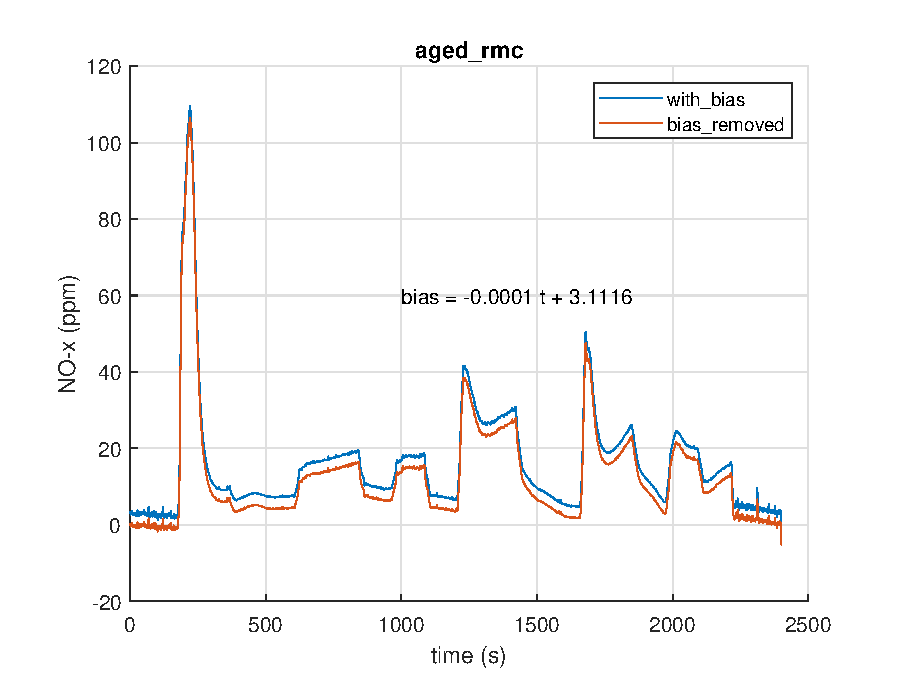
\includegraphics[width=\textwidth]{./figs/chi_est/aged_rmc_NOx_bias.eps}
        \end{figure}
    \end{minipage}
    \begin{minipage}{0.4\textwidth}
        \begin{figure}[H]
            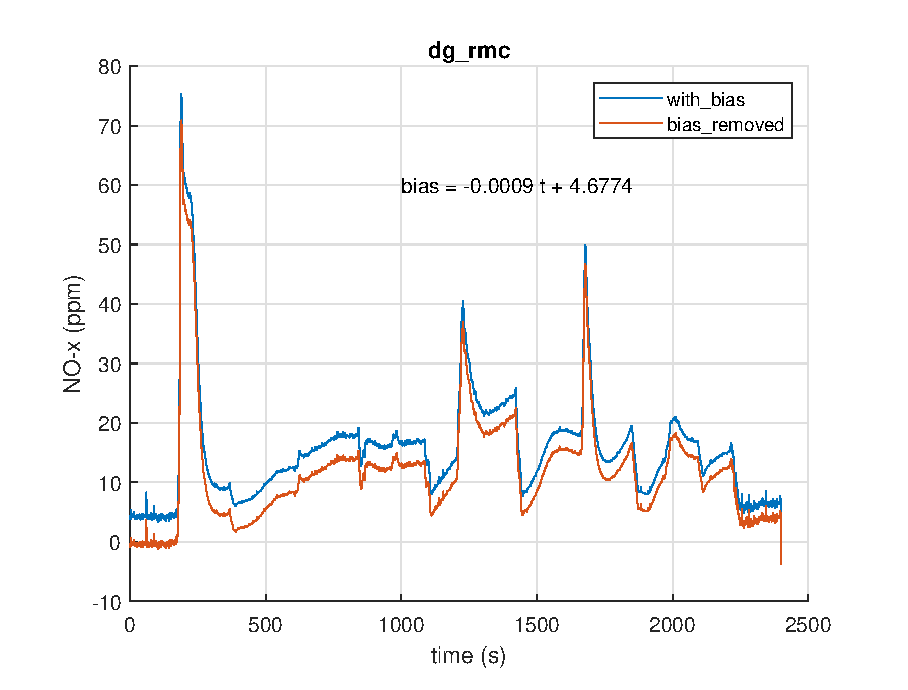
\includegraphics[width=\textwidth]{./figs/chi_est/dg_rmc_NOx_bias.eps}
        \end{figure}
    \end{minipage}
        \caption{Sensor bias correction for RMC cycles}
\end{figure}



\subsubsection{Effect of $NH_3$ sensor bias and minimum threshold for cross-sensitivity}

The ammonia sensor used for ammonia measurement also has bias and there is a
threshold for ammonia sensor for cross-sensitivity to be effective. Thus the
expression for cross-sensitivity becomes:
\begin{align*}
    y_1 &= x_1 + \chi (x_2 - x_{2_{th}})\\
    \implies y_1 &= \bm{x_1 & x_2 & -1} \bm{ 1 \\ \chi \\ \underbrace{\chi \lr{x_{2_{th}}}}_{b}}
\end{align*}

\subsubsection{Least-squares estimation}
\itbf{Assumption}: The temperature changes in RMC cycle don't effect the
cross-sensitivity factor significantly. Thus it can be treated as a constant
w.r.t temperature fluctuations in that range.

We have,
\begin{align*}
    \underbrace{y_1 - x_1}_{\pmb y} &= \underbrace{\bm{x_2 & -1}}_{\pmb \phi^T} \underbrace{\bm{ \chi \\ b}}_{ \pmb \theta}\\
\end{align*}


\subsubsection{Conclusions}
The full non-linear model for gas concentrations was derived based on a CSTR
model with reduced-order dynamics, that were previously justified in
literature. Model parameters were determined as explicit functions of reaction
rates and the catalyst's ammonia storage capacity.  Parameter identification,
beginning with the output equation and focusing on $NO_x$ sensor
cross-sensitivity ($\chi$), was carried out using RMC test-cell data from
degreened and aged catalysts. A preliminary indicator of aging was observed
from the catalyst's storage capacity versus temperature curve.

\section{Research Objectives and Scope}
\subsection{Approach to the research problem}
Our approach is based on the presumption that the aging detection problem can be framed as a state/parameter estimation challenge with respect to the concentration dynamics of the gases involved. This gives rise to the following sub-problems:

\begin{enumerate}
\item Determining a suitable model for the system dynamics.
\item Assessing whether the available data contains sufficient information for identifying the model parameters related to the chosen system dynamics.
\item Investigating the relationship between the parameters/states and the aging factor of the catalyst.
\item Understanding the uncertainties inherent in the aforementioned processes.
\item Finally, developing and validating the aging detection algorithm.
\end{enumerate}

\subsection{Objectives for 2023 (previously)}
\begin{enumerate}
 \item In the current data, the operating conditions in the truck cover a wider range than the ones in test-cell. So, we wish to validate the SCR-ASC model on test-cell data with operating conditions similar to the truck data. If it is difficult to obtain such experimental data in test-cell, then use a high-fidelity SCR-ASC model in AVL Boost, to validate our low fidelity diagnostics-oriented model across a wide range of transient and steady operating conditions.
 \item Explore other low fidelity diagnostics-oriented SCR-ASC model structures, that could be calibrated using the signals between SCR and ASC that could be obtained from the high-fidelity Boost model.
 \item Validate the model-based and data-driven OBD results using truck data from trucks with DG and/or an EUL catalyst.
 \item Validate the model-based and data-driven OBD results using high-fidelity simulations.
 \item Based on the model and OBD validation results, iterate and improve both model-based and data-driven approaches to achieve robust diagnostics performance validated using high-fidelity simulations and actual data. Also implement a more rigorous and detailed version of the stochastic model-based OBD.
 \item Support TTU in development and demonstration of model-based, data-driven, and frequency-domain OBD methods that rely on detecting NOx-rich regions where ASC is inactive.
\end{enumerate}


\subsection{Objectives for 2024}
\begin{enumerate}
\item Identify the model parameters and parametric uncertainties using
the test-cell data and data from AVL boost model and validate them.
\item Develop the estimation methodology for the storage capacity (Observer Design).
\item Relate catalyst's aging to the storage capacity and develop robust
non-intrusive aging detection algorithm and test the algorithm on the test-cell
data and the road data segments.
\end{enumerate}
\subsection{Objectives post-2024}
\begin{enumerate}
    \item Assess the potential to embed the algorithms for real-time computation.
    \item Implementation and comprehensive evaluation, including robustness analysis, of the proposed diagnostic algorithms in engine test cell and on the road.
\end{enumerate}


\subsection{Other requirements}
\begin{itemize}
    \item Prior to the end of this project, a proposal for follow-on work will be submitted to Cummins.
    \item Cummins to provide expertise via mentorship and regular feedback.
    \item Cummins to provide funds to support the students.
    \item Cummins to provide test-cell data with operating conditions similar to on-road trucks
    \item Cummins to provide truck data with at least one and preferably two known aging levels (could be DG and/or EUL)
    \item Cummins to provide access to high-fidelity AVL Boost model for SCR-ASC. This could be a black-box model with access to pre-SCR, post-SCR, post-ASC signals, and NH3 storage values in SCR and ASC.
\end{itemize}

\section{Intellectual Property}
(Select)
\begin{itemize}
    \item Track 1 - CNERF (8.4.1)
    \item Track 2 - 5-Year Exclusive License (8.4.2)
    \item Track 3 - Work-for-Hire - IP Assignment (8.4.3)
\end{itemize}

\section{Publication}
{\color{red}(Select)}
\begin{itemize}
    \item  Publication Review
    \item Publication Approval (Requires Purdue Export Control Technology Control Plan) (8.6.3)
\end{itemize}

\section{Timeline and Deliverables}
\subsection{Timeline for 2024}

\begin{table}[H]
    \centering
    \begin{tabular}{l l l}
        \hline\hline
                & Task & $|$Quarter1$|$Quarter2$|$Quarter3$|$Quarter4$|$ \\\hline\hline
        1.      & Model parameter identification   & $|++++|----|----|----|$\\
        2.      & Validating identified model      & $|--++|++--|----|----|$\\
        3.      & Formal definition of aging factor& $|----|--++|----|----|$\\
        4.      & Algorithm development            & $|----|----|++++|++--|$\\
        5.      & Validation                       & $|----|----|----|++++|$\\
        \hline\hline
    \end{tabular}
\end{table}
\subsection{Deliverables}
The deliverables for the research project will be in the form of documentation
and the code for processing data and validation of algorithms.

\begin{enumerate}
    \item The documentation includes:
\begin{enumerate}
    \item Detailed system model derived from the first principles with assumptions.
    \item Model parameter estimation methods and the results of such endeavor.
    \item Formal definition of aging factor estimation problem.
    \item Aging factor estimation algorithm and validation results.
\end{enumerate}

\item The code repository will include routines for:
\begin{enumerate}
    \item Model parameter estimation and validation using test-cell data.
\item Programs for handling the AVL boost simulation model provided for model
parameter identification purposes.
\item Aging factor estimation for test-cell and truck data and validation using
test-cell data.
\end{enumerate}

\end{enumerate}

\section{Budget}

\begin{table}[H]
    \centering
    \begin{tabular}{l l}
        & Year 2024\\
    Personnel Costs:    &\\
	Travel:             &\\
    S$\&$E:             &\\
    Indirect Costs:     &\\
    TOTAL:              &\\
    IP Fees:            &
    \end{tabular}
\end{table}
\begin{flushright}
    Grand Total : $\_\_\_\_\_\_\_$
\end{flushright}

Cummins will generate a PO for each year of the approved Research Project Plan
to facilitate annual payments provided at the beginning of each project year.\\

\noindent \textbf{PURDUE RESEARCHER}: Prof. Peter H. Meckl\\

\noindent \textbf{CUMMINS PRINCIPAL INVESTIGATOR}: Lyle E. Kocher\\


\noindent \itbf{By signing below, the parties authorized representatives agree to this Research Project Plan.}

\begin{table}[H]
    \centering
    \begin{tabular}{l c l}
        \itbf{CUMMINS, INC.} & $\qquad$ &\itbf{PURDUE UNIVERSITY}\\
        By:$\_\_\_\_\_\_\_\_\_\_\_\_\_\_\_\_\_\_\_\_\_\_\_\_\_\_\_\_\_$ & $\qquad$ &
        By:$\_\_\_\_\_\_\_\_\_\_\_\_\_\_\_\_\_\_\_\_\_\_\_\_\_\_\_\_\_$ \\
        Printed Name : & $\qquad$ & Printed Name:\\
Title:$\_\_\_\_\_\_\_\_\_\_\_\_\_\_\_\_\_\_\_\_\_\_\_\_\_\_\_\_\_$ &	$\qquad$
&Title:
                $\_\_\_\_\_\_\_\_\_\_\_\_\_\_\_\_\_\_\_\_\_\_\_\_\_\_\_\_\_$ \\
Date: $\_\_\_\_\_\_\_\_\_\_\_\_\_\_\_\_\_\_\_\_\_\_\_\_\_\_\_\_\_$ & $\qquad$ &
Date: $\_\_\_\_\_\_\_\_\_\_\_\_\_\_\_\_\_\_\_\_\_\_\_\_\_\_\_\_\_$\\
    \end{tabular}
\end{table}



\newpage
\bibliographystyle{unsrt}
\bibliography{refs}

%===============================================================================
\newpage
\begin{center}
    APPENDIX B\\
    \bigskip
    PROJECT PAYMENT
\end{center}


The Sponsor agrees to pay the Total Project Cost and Project IP Fees set forth
in Appendix A upon acceptance and approval of an Appendix A - Research Plan.
Sponsor will generate a PO for each year of the approved Research Project Plan
to facilitate annual payments provided at the beginning of each project year.


The invoices for the payment of Project will be sent to:

\begin{table}[H]
    \centering
    \begin{tabular}{l l}
        Contact Person: & Cummins Inc.\\
        Address: & Business Services PO Box 290909, Nashville, TN  37229-0909 \\
        Phone: & \\
        Secondary Contact: & \\
        Email/E-Invoice: &
    \end{tabular}
\end{table}

\underline{Payments by Check}:

Payments will be made to Purdue University and mailed to:
\begin{table}[H]
    \centering
    \begin{tabular}{l}
        Purdue University\\
        Sponsored Program Services\\
        23510 Network Place\\
        Chicago, Illinois 60683-1235
    \end{tabular}
\end{table}


\underline{Payments by ACH and Wire}:

Purdue University's bank account details for ACH and WIRE payments is listed
below:
\begin{table}[H]
    \centering
    \begin{tabular}{l l}
        Bank Name: 		    &JPMorgan Chase Bank, N.A.\\
        Account Title: 		&Purdue Incoming Electronic Payment ZBA\\
        Account Number: 	&5157579\\
        &\\
        \textbf{Wire Detail}:&\\
        Street Address: 	&270 Park Avenue, New York, NY 10003\\
        Routing Number: 	&021000021\\
        Swift Code: 		&CHASUS33\\
        &\\
        \textbf{EFT/ACH Detail}:&\\
        Street Address: 		&10 S. Dearborn Street 36th Floor, Chicago, IL 60603\\
        Routing Number: 	&071000013
    \end{tabular}
\end{table}

Any payment related questions or concerns should be directed to spscash@purdue.edu.\\

The memorandum section of the wire \textbf{\underline{must}} specify the invoice number or award number. Purdue University only accepts wires in U.S. Dollars. Electronic transactions may be returned within 45 days if the transaction information is insufficient.

\newpage
%===============================================================================
\begin{center}
    APPENDIX C\\
    \bigskip
    ASSIGNMENT
\end{center}

\end{document}
